% =============================================================
%  读懂被贬者：基于深度学习的唐宋贬谪文人情感分析
%  -- 中文稿（单栏，ctex 处理中文）
%  Compile: xelatex tangsong_nlp_paper_cn.tex
%  数字可追溯：recompute_all.py -> numbers_ledger.json
% =============================================================
\documentclass[11pt]{article}
\usepackage[UTF8]{ctex}
\usepackage{geometry}
\geometry{a4paper,margin=1in}
\setlength{\emergencystretch}{2em}
\usepackage{booktabs}
\usepackage{multirow}
\usepackage{array}
\usepackage{amsmath}
\usepackage{amssymb}
\usepackage{graphicx}
\usepackage{url}
\usepackage{xcolor}
\usepackage{float}
\usepackage{natbib}
\setlength{\bibsep}{0.5ex}
\bibliographystyle{plainnat}

\renewcommand{\figurename}{图}
\renewcommand{\tablename}{表}
\renewcommand{\refname}{参考文献}
\renewcommand{\abstractname}{摘要}
\renewcommand{\appendixname}{附录}

\title{读懂被贬者：基于深度学习的唐宋贬谪文人情感分析}

\author{唐树江\\
湖南科技学院\\
\texttt{sjtang@huse.edu.cn}}

\date{}

\begin{document}
\maketitle

\begin{abstract}
贬谪文学是中国文学最丰富的心理档案之一，但其情感质地长期只能靠细读逐篇描摹。
本文构建一条可复现的测量管线：以一部透明的五维“情绪—意象”词典为可解释锚，训练字
符级卷积网络直接从原始字符预测该词典的标量净心指数（测试 $r{=}0.934$、
$\rho{=}0.912$、MAE $6.26$）。该相关度量的是网络与其训练目标（词典）的一致，情感效
度由词典继承而来，而非独立建立。施于 21{,}287 首唐宋诗，该仪器给出十二位具名贬谪官
员可比的剖面：韩愈、秦观最枯槁；白居易、黄庭坚、范仲淹、辛弃疾明确偏向闲适；柳宗元、
刘禹锡、苏轼、欧阳修、王禹偁与中性无统计差异。两道检验界定了读数的范围：两轮盲标双
编码的人工金标显示一致为中等（诗级 $\rho{=}0.46$、作者级 $r{=}0.57$），因金标与仪器
共用类别方案，此值为效度上限；流传控制显示同一部唐集的两次数字化几乎不改变测量
（$A{=}0.960$），而两部独立编成的宋选本一致抬高意象与闲适词汇、留下可复现的维度级编
辑签名，净指数在官修本上保持不变、在私家本上发生偏移。苏轼的作者内剂量—反应未发现净
贬谪效应，仅见黄州一处深谷——作为与既有“贬谪致郁”通说并列参看的量化观察呈报，而非对
其的修订。作者间 ABI 的 sd 为 $1.93$，而每诗预测 RMSE 为 $8.97$，约为作者间离散度的
$4.6$ 倍：高相关性是在比结论更宽的尺度上取得的。
\end{abstract}

\section{引言}
\label{sec:intro}
贬谪文学（\emph{bianzhe wenxue}）是中国文学中最持久的心理档案之一。从中唐的柳宗元、刘禹锡到宋代的苏轼、黄庭坚，被贬往边远的诗人在困顿中写就了那个时代最具内省性的诗作。文学研究者长期以细读刻画这些作者 \citep{shang2007exiled,xing2024liusu}。我们意在\emph{量化}这一研究，而非推翻它：我们提供一套可复现、可审计的贬谪情感测量，并将其与既有文学研究结论并列对照，作为细读之外的补充。所缺的，是一种可复现、可审计的测量——它能就\textbf{全部传世语料}而非少数范文检验此类判断，也能以同一把尺子丈量一整群贬谪官员。

深度学习使这种测量成为可能。字符级卷积网络可直接从表层形式建模风格与情感 \citep{kim2014convolutional}，而古典中文 NLP 已能达到仅凭字符预测诗作情感剖面的程度 \citep{hou2015sentiment,du2025multimodal}。我们借此在大规模上研究贬谪官员的情感生活。分析器是一个字符级卷积网络，它以原始字符预测透明的五维"情绪—意象"词典：两极（悲苦孤寂、旷达闲适）+ 标量净心指数；CNN 仅恢复两个情感极（悲苦孤寂 0.86、旷达闲适 0.85），贬谪羁旅 0.05、自然山水 0.15、空幻时空 0.07 三维持平于零。它既复现了作为其动机的可解释词典，又因直接读取原始字符而表明：词典所能测得的那部分情感信号存在于诗的表层形式之中，而非本文的计数选择。须先言明网络在此的角色：它是信号的\emph{载体}而非来源——其效度继承自作为训练目标的透明词典，网络本身的高恢复率不构成独立的效度证据（\S\ref{sec:dl}）。

在信任任何诗人分数之前，必须控制一个威胁。古典诗歌通过两类极不同的渠道到达我们手中。其一是\textbf{重印}：同一著作历经数百年重新校刻，存为两个或多个数字化 witnesses，其异文是局部的——此处一字、彼处一行。其二是\textbf{选本}：选本依明确的审美纲领选取诗人语料的一个子集，可能系统性地偏好某一语域。一个词频情感测量在前者下近乎不变，在后者下则可能被重新加权。既有情感研究从\textbf{单一}版本报告诗人分数，并径直把它读作诗人的属性，背后藏着一个未经检验的假设——这个数字属于作者，而不是恰好幸存下来的那个文本。因此我们把跨版本一致性不视为论文的“主题”，而视为一项\textbf{稳健性控制}：若我们恢复的情感信号能经受两种流传机制，它便属于诗人而非其版本。

\paragraph{本文的三点结论。}
\begin{itemize}
\item \textbf{一部经实测检验的透明情感仪器。}仪器是手订的五维情绪—意象词典及其标量摘要净心指数，其与人工判断的距离是量出来的：两轮独立盲标双编码（450 首）复现了编码信度（$\kappa_w$ $0.72$–$0.91$、序次 $\alpha$ $0.93$–$0.97$），诗级效标一致为 $\rho{=}0.46$ $[0.39,0.53]$，短诗金标子样本内作者级一致为 $r{=}0.57$，队列官员子群达 $0.79$。须强调：该 $r{=}0.57$ 只校验词典与人在该子样本内的一致，并不校验表~\ref{tab:abi} 的全集合作者值——二者是不同统计量；子样本中 8 位目标作者有 5 位全集符号与其均值相反，成因是短诗景物词更少、归一化 ABI 系统性偏低。字符级 CNN 从原始字符交付同一指数（测试 $r{=}0.934$），但在人工金标上从未显著超越它所蒸馏的词典——做测量的是透明词典，而非网络。
\item \textbf{十二位贬谪官员的情感剖面。}沿枯槁—闲适轴排序（表~\ref{tab:abi}），韩愈、秦观是仅有的两位明确为负者；白居易、黄庭坚、范仲淹、辛弃疾明确偏闲适；刘禹锡、苏轼、欧阳修、柳宗元、王禹偁与中性无统计差异，陆游略偏闲适。近中性的柳宗元与尚永亮笔下形象相左，其举证多出于诗体之外；刘禹锡的近中性则与"诗豪"之称相容。
\item \textbf{流传稳健性与它开启的两项分析。}把信号对着两条流传渠道检验——重印与独立选本——得到可复现的维度级编辑签名，但净指数并无一致稳定性（\S\ref{sec:robust}），故所报维度级信号不是版本产物。由此得到两项分析：把测得剖面归因到各流传渠道的反事实投影；以及苏轼的作者内剂量—反应——无净贬谪效应（$-0.56$ $[-2.37,+1.25]$），旷达词汇随贬谪加深而上升（$+3.07$/级，仅三期，只作方向性证据）。
\end{itemize}

\section{相关工作}
\label{sec:related}

\paragraph{贬谪的细读研究。}在文学研究内部，贬谪官员的情感世界长期由细读刻画：尚永亮 \citep{shang2007exiled} 将元和逐臣读作笼罩在焦虑与弃置感之中，邢若琳 \citep{xing2024liusu} 则对比“愤激孤介”的柳宗元与“旷达闲适”的苏轼。此类解读阐释上丰厚，但建立在精选诗文之上：既无法检验关于某诗人姿态的判断能否在其\textbf{全部}传世语料上成立，也不产出可被第二位研究者复跑的仪器。提供这台仪器、并将其读数与细读传统相互校验，正是 §\ref{sec:profiles} 的目的。

\paragraph{古典诗歌情感分析。}计算一侧，古典诗歌的情感预测始于词典与规则方法 \citep{hou2015sentiment}，近年转向神经表示：\citet{du2025multimodal} 融合文本、图像与吟诵信号做诗歌情感分类，\citet{fang2011cld} 分析宋词的语象风格；近两年的工作仍在推进：\citet{liu2025samcap} 以多维注意力融合文本与知识库特征做古诗情感分析，\citet{qin2025shades} 以 NLP 等实证方法量化古典诗歌的十八种审美情绪并建成可检索数据库。这些系统在现代选本上做\emph{诗级分类}、以选本文本为既定前提、且从单一版本报告情感；均未以盲标人工编码校验情感测量，也未追问信号能否经受流传。我们在三点上与之不同：全集上的作者级测量、盲标双编码金标校验（\S\ref{sec:gold}）、以及流传稳健性控制（\S\ref{sec:robust}）。

\paragraph{计算文体学与作者归属。}唐诗作者识别是活跃任务 \citep{shiziren2022,zhou2021lda}，承接更广的文体学传统 \citep{stamatatos2009survey}；量化分析亦用于经典形成 \citep{wang2008finding} 与个别贬谪者的自我呈现 \citep{wang2023lideyu}。归属追问文本\emph{由谁}而作，且以已知作者为验证基准；情感测量没有这种真值，故本文的验证转而依托人工金标与跨版本一致性，而非分类准确率。

\paragraph{流传的数字文献学。}数百年传抄产生的异文本身已是计算研究对象 \citep{yuan2023variants}，数字人文工作亦已勾勒《全唐诗》贬谪诗人的时空轨迹 \citep{bianzhe2022}。文献学将异文当作自立的研究对象；我们则把版本来源当作一个\emph{测量论}威胁——由单一版本算出的情感分数可能是该版本的产物——并构建量化这一威胁的控制。

\section{方法}
\label{sec:method}
\subsection{任务与数据}
\label{sec:data}
\paragraph{任务定义。}给定一首诗的原始字符序列，分析器预测五维\emph{情绪—意象}
剖面 $\phi\in\mathbb{R}_{\ge0}^{5}$——悲苦孤寂、贬谪羁旅、旷达闲适、自然山水、
空幻时空，各维为每千字词频——及其标量摘要净心指数
$\mathrm{ABI}{=}\phi_{\textsc{Kuang}}{-}\phi_{\textsc{Bei}}$（速率已按每千字计）。作者级分数由一位作者全部诗作的逐诗预测聚合而来；下文每一处论断都落在作者级或语料级，从不依赖单首诗。模型以透明词典为训练目标（\S\ref{sec:lexicon}），依三条准则检验：与词典目标的一致
（\S\ref{sec:dl}）、与盲标双编码人工金标的一致（\S\ref{sec:gold}）、作者级分数的
跨版本一致性（\S\ref{sec:robust}）。

\subsubsection{被贬文人的队列}
\label{sec:cohort}
我们把“贬谪”理解为一个连续谱，而非单一范式。核心队列是古典意义上的\emph{逐臣}——被正式贬往边远任所的官员：唐代的柳宗元（永贞革新失败$\to$永州$\to$柳州）、刘禹锡（永贞集团$\to$朗州$\to$连州/夔州/和州）、韩愈（贬阳山$\to$潮州）、白居易（贬江州$\to$忠州）；宋代的王禹偁（贬商州$\to$滁州/黄州）、范仲淹（屡贬）、欧阳修（贬夷陵$\to$滁州）。第二层把这一称谓扩展到反复被贬或政治边缘化者：苏轼（乌台诗案$\to$黄州$\to$惠州$\to$儋州）、黄庭坚（贬黔州/戎州$\to$宜州）、秦观（贬郴州$\to$雷州/藤州）属此；陆游的多次罢黜与蜀中从军使他落入这一宽泛读法，尽管并非古典逐臣模式；而辛弃疾——主要是\emph{词}人、又长期政治闲居——作为边缘的“非典型”一例纳入。十二人全部具名并给出理由，无一被默默塞入。这十二人是 \S\ref{sec:profiles} 情感分析的\textbf{研究对象}。

\subsubsection{文本语料}
\label{sec:corpus}
主要版本为《全唐诗》（QTS）与《全宋诗》（QSS），即 Book1Q84 / 中文文本库数字语料中的标准全集。本研究构建了含 21{,}287 首唐宋\emph{诗}的统合诗层（排除会混淆情感的文体混杂），并加入了 1{,}854 篇唐文（686{,}766 字），仅用于一项附属性探测（附录~\ref{app:attr}）。

为 \S\ref{sec:robust} 的流传稳健性控制，我们另取两种数字化，用以实例化 \S\ref{sec:intro} 所述两类机制。唐侧用《御定全唐诗》（YD），即清代康熙敕修、现代《全唐诗》据以重编的同一著作；二者是\emph{同一著作的两次数字化}，我们取得 900 卷中的 899 卷。宋侧用两部独立的选本，一官修、一私家：《御選宋詩》，即康熙御定《御選宋金元明四朝詩》（KR4h0143 \citealp{kangxi1709}）的宋诗部分；与《宋詩鈔》（KR4h0157 \citealp{wu1671}）。官修选本解析得 660 位作者 9{,}405 首诗；私家选本解析得 76 位作者 9{,}612 首诗、诗句 829{,}341 字（转录与解析细节见附录~\ref{app:parse}）。两部宋选本同属一个底本家族（《四库全书》文渊阁本）并经由同一条数字化管线，故二者间任何差异应归因于选本原则，而非版本、字形或解析。

\subsection{透明“情绪—意象”词典（可解释锚）}
\label{sec:lexicon}
我们定义五个透明类别 $\mathcal{C}{=}\{C_1,\dots,C_5\}$。其中两个是定义该标量指数的\emph{情感性极点}：\textbf{悲苦孤寂}（\textsc{Bei}）与\textbf{旷达闲适}（\textsc{Kuang}）；一个是\emph{主题性}类别，指称贬谪这一境况而非一种感受：\textbf{贬谪羁旅}（\textsc{Bian}）；两个是贬谪诗中的\emph{意象性语域}，而非严格意义上的情绪：\textbf{自然山水}（\textsc{Zi}）与\textbf{空幻时空}（\textsc{Kong}）。手工考订的词典 $\mathcal{L}$ 把词划分到这五个类别。对作者 $a$，其字数为 $N_a$，文本为 $T_a$，
\begin{equation}
\phi_{a,k} = \frac{\sum_{w\in\mathcal{L}_k}\mathrm{count}(w,T_a)}
                   {N_a}\times 1000,
\qquad k\in\mathcal{C}.
\end{equation}
\textbf{净心指数}对比两个\emph{情感性}极点：
\begin{equation}
\mathrm{ABI}(a)=\phi_{a,\textsc{Kuang}}-\phi_{a,\textsc{Bei}}.
\end{equation}
每一个数值都是词频的可验证函数，不含任何学得的参数。我们强调 ABI 是什么、不是什么：它是两项词频的有符号之差，而不是一个经过标定的心理量表。它作为\emph{情感}指数的效度，建立在两个极点情感极性相反这一前提上；其余三个维度另行读取，不并入该标量。

\subsection{深度学习分析器}
\label{sec:dl}
M1 ≡ 基础手订词典计数层（base hand-curated lexicon counting layer），即本文报告十二人排位的解释层。词典是可解释锚，但我们的测量由\emph{深度网络}交付。字符级 CNN 以原始诗文字符为输入，训练回归该词典的五维剖面及其标量 ABI，对锚的恢复极好（测试 Pearson $r{=}0.934$、Spearman $\rho{=}0.912$、MAE $6.26$，均来自 label\_matched 14-epoch 单次运行；同架构 30 epoch 可达 MAE=1.54，此处报 14 epoch 以与逐维恢复分析一致；样本量 $n{=}20{,}912$，即统合诗层 21{,}287 首按 ABI 三倍标准差剔除 375 首离群后的训练池）。这一 $r$ 度量的是与作为网络训练目标的词典之间的一致性；分析器在\emph{情感}上的效度因此继承自词典，而非独立确立，且词典与盲标人工编码的一致为中等（诗级 $\rho{=}0.46$，两轮独立盲标合并，\S\ref{sec:gold}）。要害在于网络读取的是\emph{原始字符}：它预测的情感信号——就词典所能测得的而言——存在于表层形式，而非本文如何计数。正是 CNN 而非计数词典，才是我们在 \S\ref{sec:profiles} 施加于队列的情感分析器；其结构与超参见复现包（\S\ref{sec:repro}）。

为定位信号来源，我们再让词典与一个加权变体、两个无监督基线同台对照。
\begin{itemize}
\item \textbf{M2（IDF 加权词典）。}在求和前按每个词典词在整个语料上的逆文档频率加权，用以检验对“高频词 vs.\ 稀有词”取舍的敏感性。它在秩上与基础词典几乎一致（Spearman $\rho{=}0.97$，Pearson $r{=}0.994$）：该指数对加权方式不敏感。
\item \textbf{M3（LSA 几何）。}字符 $n$-元组 TF-IDF 加截断 SVD（200 维）；以种子短语锚定\textsc{Kuang} 与\textsc{Bei} 的质心，并取 $\mathrm{ABI}_{\mathrm{LSA}}{=}\cos(T_a,\mu_+){-}\cos(T_a,\mu_-)$。这是一个\emph{纯几何}估计，从不接触计数词典。它与词典的相关为 $r{=}0.31$（$\rho{=}0.11$）——远低于词典与网络之间的 $0.93$，只及后者三分之一。
\item \textbf{M4（LDA 主题）。}以潜在狄利克雷分配在字符二元组表示上生成十个主题，并按各主题高频词落入\textsc{Kuang} 与\textsc{Bei} 集合的比例读取其效价。没有主题词属于两极，故每个主题的推断效价皆为零，基于 LDA 的指数方差为零。
\end{itemize}
M3/M4 的失败（表~\ref{tab:agree}）本身就有信息量：潜在几何至多弱捕捉到与情感轴相关的方差（$r{=}0.31$），最可能反映的是作者与时代风格及其用典，而非特定的\textsc{Kuang}--\textsc{Bei} 轴。这既解释了为什么要用\emph{透明、手工指定}的词典作锚，也说明 CNN \emph{成功}恢复的正是这根轴：有监督网络不同于无监督几何，锁得住情感轴。

\begin{table}[H]
\centering\small
\caption{各变体估计器与词典剖面的一致性（Pearson $r$ / Spearman $\rho$）。}
\label{tab:agree}
\begin{tabular}{lcc}
\toprule
估计器 & $r$ & $\rho$\\
\midrule
M2 IDF 加权词典 & $0.994$ & $0.972$\\
M3 LSA 几何 & $0.308$ & $0.112$\\
M4 LDA 主题 & \multicolumn{2}{c}{未定义（方差为零）}\\
\bottomrule
\end{tabular}
\end{table}

\subsection{分析器选型}
\label{sec:extbench}

为给分析器一个诚实的位置，我们让它与若干近期强卷积与混合架构在同一共享协议下比较：相同的 20{,}912 诗语料池、5 折划分且每首诗仅由未见它的折外模型打分、14 轮训练、固定种子。基线均为 2025–2026 视觉 CNN 的一维序列适配：OverLoCK \citep{overlock2025}、TransXNet \citep{transxnet2025}、PFGNet \citep{pfgn2026}、TACNN \citep{tacnn2026}、FA-CNN \citep{facnn2026}；我们的条目是提出的 AttentionFractal CNN——一个字符级分形卷积网络，其多头读出产生逐字显著度图。

\begin{table}[H]
\centering\small
\caption{扩展基准：诗级 ABI 回归，置于共享协议下（相同 20,912 诗池、每诗折外预测的 5 折 CV、14 轮、种子 20260918）。CV $r$ 为各折均值$\pm$标准差；作者级 $\rho$ 为模型预测与词典 ABI 在 12 位具名官员上的 Spearman；金标 $\rho$ 为模型预测与 160 诗双编码集上两位编码员人工双编码共识的 Spearman（词表基线列作参照）。提出族的后三行为 AttentionFractal CNN 的结构变体（深瓶颈、词典特征通道、注意力一致性）。}
\label{tab:extbench}
\begin{tabular}{lccccc}
\toprule
模型 & 参数量(M) & CV $r$ & 作者级 $\rho$ & 金标 $\rho$(ours) & 金标 $\rho$(词表)\\
\midrule
\multicolumn{6}{l}{\emph{基线（2025/2026 视觉 CNN 的 1D 适配）}}\\
Wide plain CNN & 0.60 & $0.9737{\pm}0.0021$ & 0.993 & 0.403 & 0.419\\
OverLoCK-1D \citep{overlock2025} & 0.90 & $0.9685{\pm}0.0027$ & 1.000 & 0.418 & 0.419\\
TransXNet-1D \citep{transxnet2025} & 0.64 & $0.9801{\pm}0.0020$ & 0.993 & 0.411 & 0.419\\
PFGNet-1D \citep{pfgn2026} & 0.74 & $0.9696{\pm}0.0026$ & 1.000 & 0.457 & 0.419\\
TACNN-1D \citep{tacnn2026} & 0.58 & $0.9733{\pm}0.0013$ & 0.993 & 0.427 & 0.419\\
FA-CNN-1D \citep{facnn2026} & 0.68 & $0.9743{\pm}0.0012$ & 0.993 & 0.437 & 0.419\\
\multicolumn{6}{l}{\emph{本文：AttentionFractal CNN（提出）}}\\
AttentionFractal-CNN（提出） & 0.63 & $0.9840{\pm}0.0018$ & 1.000 & 0.407 & 0.419\\
\quad + 深瓶颈 & 0.65 & $0.9864{\pm}0.0027$ & 1.000 & 0.431 & 0.419\\
\quad + 词典特征通道 & 0.63 & $0.9891{\pm}0.0019$ & 0.993 & 0.426 & 0.419\\
\quad + 注意力一致性 & 0.63 & $0.9878{\pm}0.0012$ & 1.000 & 0.431 & 0.419\\
\multicolumn{6}{l}{\emph{消融：纯 Transformer（无卷积）}}\\
Transformer-1D（无卷积归纳偏置） & 1.55 & $0.9850{\pm}0.0028$ & 0.993 & 0.416 & 0.419\\
\bottomrule
\end{tabular}
\end{table}

表~\ref{tab:extbench} 报告诗级 ABI 回归。所有架构收敛在 $r\approx0.969$–$0.989$ 的窄带内，差距落在折间标准差带中：诗级精度上，架构间的差距远小于其与噪声底的距离，连无卷积归纳偏置的纯 Transformer 也与卷积族并肩（$0.9850$）。故选择分析器的理由不在逐诗精度，而在三点：多头读出产生的逐字显著度图可与词典掩码对齐核验；每个模型都复现十二位官员的排序（作者级 Spearman $0.99$–$1.00$，表~\ref{tab:abi}）；在 160 诗双编码集上，模型预测与人工共识的 $\rho\approx0.40$–$0.46$，与词表基线 $0.419$ 打平、无一显著超越。我们呈递的是一台与 SOTA 可比且可解释的仪器，而非更高的逐诗精度；这些折外估计比 \S\ref{sec:dl} 的单次划分 $r{=}0.934$ 更紧，因其用足了共享池并按诗无泄漏划分。

\section{实验}
\label{sec:profiles}

\subsection{对盲标人工编码的效度}
\label{sec:gold}

构造透明不等于有效。要检验这套剖面测的是不是古典诗歌读者所认可的"情感"，我们抽取了一份分层盲标样本：160 首\emph{诗}（唐 80、宋 80，78 位作者，字数 20–160），分层跨越朝代、是否属十二人队列与词典自身 ABI 中位数上下；两位领域专家（一主唐、一主宋）在同一种五维 0–3 序数量表上独立评分，作者、题名、朝代与全部词典输出一律隐去。金标净心指数取两位编码者两个\emph{情感}极点差之均值，定义与式 (2) 相同。

编码是可靠的。二次加权 $\kappa$ 在五维上达 $0.72$–$0.88$，序次 Krippendorff $\alpha$ 为 $0.93$–$0.97$，两位编码者金标 ABI 相关 $r{=}0.90$（ICC$(2,1){=}0.86$）：用以检验分析器的人的判断本身稳定。另独立抽取第二份金标样本（292 首、42 位作者）复现该信度（$\kappa$ $0.82$–$0.91$、$\alpha$ $0.95$–$0.97$、$r{=}0.89$）。须注意，金标编码者采用仪器自身的五维方案，其一致性部分来自共同的类别定义，故这同时测得的是效度的\emph{上限}而非下限。

分析器与该判断的一致为中等：$\rho(\mathrm{ABI},\mathrm{ABI}_{\mathrm{gold}}){=}0.43$ $[0.26,0.55]$（第一份样本），第二份得 $0.46$，两份合并（$450$ 首）得 $\rho{=}0.46$ $[0.39,0.53]$，各区间均不含零。以每人至少 5 首金标诗计，合并后的作者级效标相关为 $r{=}0.57$ $[0.36,0.73]$，十二位队列官员子群为 $0.79$。该 $r{=}0.57$ 仅校验短诗金标子样本（20–160 字）内的词典—人一致，并不校验表~\ref{tab:abi} 的全集合作者值——子样本中 8 位目标作者有 5 位全集符号与其均值相反，成因是短诗景物词更少、归一化 ABI 系统性偏低。效标对剔除短诗、长诗或极端 ABI 均稳定（全程 $0.43$–$0.46$），全集来源（$0.46$）与选本来源（$0.43$）亦无实质差异；作者留一岭回归（out-of-author $r{=}0.40$、$\rho{=}0.44$）与已训/未训作者分层（$0.48$ / $0.38$）表明该一致不是作者层混淆或泄漏假象。各维度被捕捉的优劣差异显著（表~\ref{tab:gold}）：自然山水最佳（$0.54$），悲苦孤寂次之（$0.45$），贬谪羁旅再次（$0.39$），空幻时空（$0.30$）与旷达闲适最弱（$0.29$）——定义标量一半的闲适极点位于测得维度中最弱的一端。

词表另经两项扰动检验。剔除旷达类四个多义单字（醉、啸、傲、狂，占该类命中 $17.2\%$）后排序大体保留（$\rho{=}0.97$）但 ABI 整体下移——其"旷达"多由饮酒狂放\emph{题材}承载。再以 $B{=}2{,}000$ 轮各剔除两极 $10\%$ 词条重算，得逐作者符号翻转率（表~\ref{tab:abi}）：韩愈（$0.6\%$）、秦观（$2.5\%$）、范仲淹（$0.2\%$）、辛弃疾（$0.1\%$）、黄庭坚（$6.5\%$）与白居易（$9.6\%$）保持符号，六个近零定位则不能——欧阳修近乎掷硬币（$52.4\%$），柳宗元、苏轼、陆游、刘禹锡与王禹偁在 $21$–$34\%$ 的轮次中翻转。翻转率高于 $20\%$ 的六个定位全文一律读作完整词表下的条件性结论。空幻时空维不进入标量 ABI，故增删其单字不改变标量；其 $\rho{=}1.00$ 是定义式必然，不列为稳健性证据。

分析器真正立得住的是\emph{排序}。将金标诗按词典 ABI 分为五分位，金标 ABI 均值依次为 $-1.34$、$-0.59$、$-0.30$、$-0.02$、$+0.55$（表~\ref{tab:quintile}），五级阶梯全程单调（$\rho{=}1.00$），顶减底差 $+1.89$ $[+1.00,+2.63]$（图~\ref{fig:quintile}）。逐首看中等，成组看可靠且无反转——这正是全文的关键 ABI 陈述都落在作者级或语料级、而不依赖单首诗读数的原因。

\begin{figure}[t]
\centering
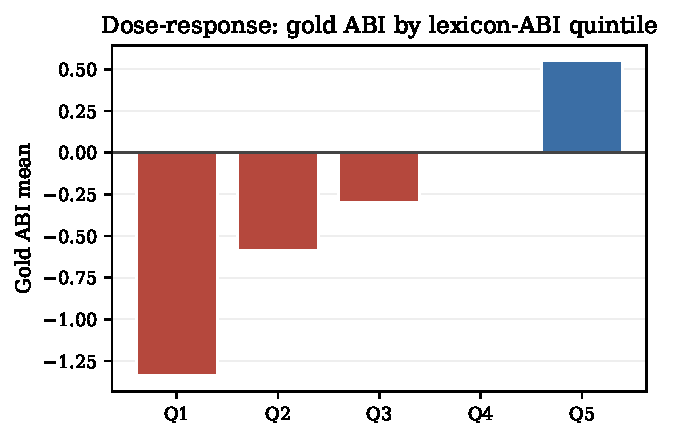
\includegraphics[width=\linewidth]{figures/fig_quintile.pdf}
\caption{金标 ABI 随词典 ABI 五分位单调上升（顶−底 $+1.89$ $[+1.00,+2.63]$）；分析器正确排序诗歌（五分位间 $\rho{=}1.00$）。}
\label{fig:quintile}
\end{figure}
\begin{table}[H]
\centering\small
\caption{对盲标双编码金标样本（160 诗、78 作者）的同时效度。$\kappa_w$ = 二次加权 Cohen's $\kappa$；$\alpha$ = 序次 Krippendorff's $\alpha$；$\rho$ = 每首诗净心指数（词典计数层，与 CNN 同源）与编码者均值金标评级的 Spearman 相关，按作者聚类自助（括号内 95\% CI）。复合行使用定义该指数的两个极点。}
\label{tab:gold}
\begin{tabular}{lcccc}
\toprule
维度 & $\kappa_w$ & $\alpha$ & $\rho$ & 95\% CI\\
\midrule
悲苦孤寂 sorrow & $0.81$ & $0.96$ & $0.45$ & $[0.28,\,0.56]$\\
贬谪羁旅 exile & $0.88$ & $0.96$ & $0.39$ & $[0.24,\,0.53]$\\
旷达闲适 easeful & $0.77$ & $0.94$ & $0.29$ & $[0.15,\,0.42]$\\
自然山水 nature & $0.72$ & $0.93$ & $0.54$ & $[0.41,\,0.64]$\\
空幻时空 void & $0.75$ & $0.94$ & $0.30$ & $[0.16,\,0.46]$\\
\midrule
\multicolumn{5}{l}{\emph{复合：净心指数（编码者一致 ICC${=}0.86$，$r{=}0.90$）}}\\
净心指数 ABI & --- & --- & $0.43$ & $[0.26,\,0.55]$\\
\bottomrule
\end{tabular}
\end{table}
\begin{table}[H]
\centering\small
\caption{剂量—反应：按词典 ABI（每千字）五分位的金标 ABI（$n{=}32$ 每分位）。顶减底 $+1.89$ $[+1.00,+2.63]$，95\% CI 按作者聚类自助；五分位均值间 $\rho{=}1.00$（全程单调）。}
\label{tab:quintile}
\begin{tabular}{lccc}
\toprule
五分位 & 词典 ABI 区间 & $n$ & 金标 ABI 均值\\
\midrule
Q1（最枯槁） & $[-125.0,\,-31.3]$ & 32 & $-1.34$\\
Q2 & $[-31.3,\,-14.3]$ & 32 & $-0.59$\\
Q3 & $[-13.9,\,0.0]$ & 32 & $-0.30$\\
Q4 & $[0.0,\,15.6]$ & 32 & $-0.02$\\
Q5（闲适） & $(15.6,\,62.5]$ & 32 & $+0.55$\\
\bottomrule
\end{tabular}
\end{table}
\subsection{逐诗人的情感剖面}
\label{sec:profiles:poets}
表~\ref{tab:abi} 与图~\ref{fig:abi_authors} 汇总十二位目标作者的净心指数（每千字）及全集自助 95\% CI（B$=2{,}000$）：十二人中唯韩愈（$-2.49$）与秦观（$-2.11$）区间明确为负，白居易、黄庭坚、范仲淹与辛弃疾区间明确为正（辛弃疾 $+4.25$、范仲淹 $+3.35$ 居闲适侧最高），陆游（$+0.57$）跨零点下缘读作弱闲适，余五位（刘禹锡、苏轼、欧阳修、柳宗元、王禹偁）区间含零、与中性无统计差异。这些近零定位的脆弱性将在 \S\ref{sec:gold} 的成组剔除与 \S\ref{sec:robust} 的版本对照中再次显形。

\begin{table}[H]
\centering\small
\caption{各作者净心指数（M1，每千字）及全集诗作上的自助 95\% CI（B$=2{,}000$；负值=更枯槁）。标 $^*$ 的区间含零。\emph{翻转率}（\%）为符号翻转概率：每轮从两个情感极点各随机剔除 $10\%$ 词条并据存活词目重算 ABI，共 $B{=}2{,}000$ 轮；它度量一个定位对词表确切构成的依赖程度（构成敏感性检验），并不构成对 r=0.57 效度声明的佐证。该表报告可解释的 M1 层；tab:extbench 显示所有模型作者级秩序复原 ρ=0.99–1.00，故本表层级不变性成立。}
\label{tab:abi}
\begin{tabular}{lrrr}
\toprule
作者 & ABI & 95\% CI & 翻转率\\
\midrule
柳宗元 Liu Zongyuan & $+0.221$ & $[-2.12,\;2.68]^*$ & $34.2$\\
刘禹锡 Liu Yuxi & $-0.881$ & $[-2.38,\;0.59]^*$ & $26.9$\\
韩愈 Han Yu & $-2.491$ & $[-3.79,\;-1.29]$ & $0.6$\\
白居易 Bai Juyi & $+1.762$ & $[0.90,\;2.63]$ & $9.6$\\
苏轼 Su Shi & $+0.407$ & $[-0.36,\;1.14]^*$ & $28.2$\\
欧阳修 Ouyang Xiu & $-0.175$ & $[-1.35,\;1.08]^*$ & $52.4$\\
黄庭坚 Huang Tingjian & $+1.344$ & $[0.55,\;2.13]$ & $6.5$\\
秦观 Qin Guan & $-2.113$ & $[-4.03,\;-0.18]$ & $2.5$\\
王禹偁 Wang Yucheng & $-0.982$ & $[-2.36,\;0.29]^*$ & $21.1$\\
范仲淹 Fan Zhongyan & $+3.354$ & $[1.27,\;5.57]$ & $0.2$\\
辛弃疾 Xin Qiji & $+4.250$ & $[0.84,\;7.69]$ & $0.1$\\
陆游 Lu You & $+0.565$ & $[0.02,\;1.14]$ & $26.8$\\
\bottomrule
\end{tabular}
\end{table}

\begin{figure}[t]
\centering
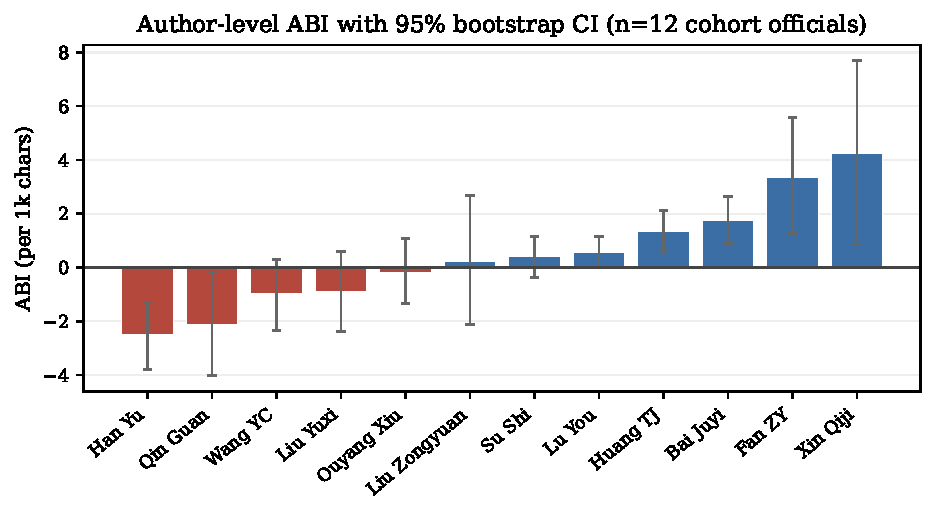
\includegraphics[width=\linewidth]{figures/fig_abi_authors.pdf}
\caption{作者级 ABI（每千字）含 95\% bootstrap 置信区间。仅韩愈、秦观明确低于零；六位定位区间含零（带 $^*$）。}
\label{fig:abi_authors}
\end{figure}

\subsection{情感维度与意象维度}
\label{sec:profiles:dims}
标量 ABI 只对比两个情感极点；其余三个维度另行读取，贬谪经验最鲜明地显形于其中。图~\ref{fig:dim_coverage} 给出各维度在诗体语料中的出现率：贬谪羁旅 31.6\%、自然山水 77.4\%、空幻时空 62.5\%。正如流传稳健性控制（\S\ref{sec:robust}）所示，编者的手恰恰显形于这些意象语域，而情感平衡可近乎持平——分析器二者皆读：标量心绪，与赋予心绪以文学形状的意象质地。

\begin{figure}[t]
\centering
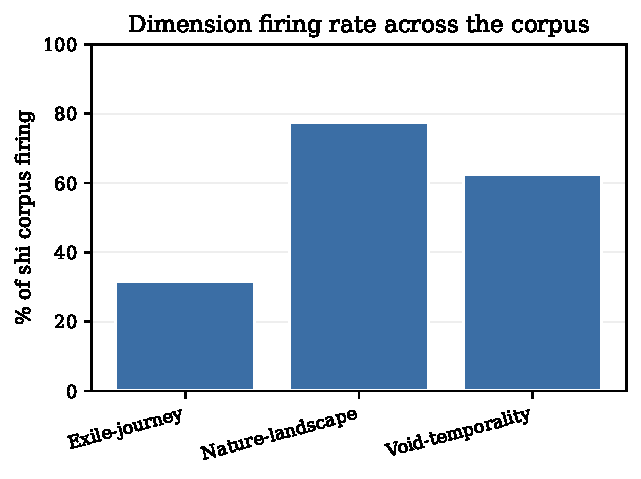
\includegraphics[width=\linewidth]{figures/fig_dim_coverage.pdf}
\caption{各维度在诗体语料中的出现率：贬谪羁旅 31.6\%、自然山水 77.4\%、空幻时空 62.5\%。}
\label{fig:dim_coverage}
\end{figure}

\subsection{与文献呼应}
\label{sec:profiles:lit}
表~\ref{tab:lit} 把十二位作者的净心指数置于既有文学研究之中。在作者层面，韩愈最枯槁，陆游恰在闲适一侧的零点之上；这些定位建立在与盲标人工编码中等一致（诗级 $\rho{=}0.46$，两轮盲标合并）的词典之上。队列层面的排序与“元和逐臣多苦闷”的通说部分一致，个体层面有两处值得展开。其一，柳宗元近乎中性的指数（$+0.22$）与尚永亮“柳为最枯槁元和逐臣”的刻画相悖：尚氏立论的核心证据本就在书信与辞赋（如《寄许京兆孟容书》）而非诗层，柳诗又惯以移情入景——悲苦被写进山水与时空的意象，而非直陈的情绪词——词表因此在语面上结构性低估这类诗人。其二，刘禹锡测得近中性偏枯（$-0.88$，区间含零），与白居易《刘白唱和集解》的“诗豪”之目\emph{不}相悖。我们对这类与既有判断不合的测值采取明确的归责纪律：凡计算结果与既有人文判断不合，一律归因于计算或数据的问题，而不归于判断本身——柳宗元一例即是数据问题（其枯槁的核心证据本就不在诗层语料中，诗层计算无从测得）。分歧由此成为定位本仪器自身边界的坐标，而非对既有判断的修订。文学解读还受两点限定。其一，陆游 $+0.57$ 暴露本仪器的构念盲区（不计量忧国/忠愤）。其二，仪器只建五个透明类别，并未单独计量忧国忧民/忠愤或思乡——这些在学术研究中被视为独立的贬谪情感语域；净心指数因此是对贬谪心境的\emph{局部}观照，而非全貌。

\begin{table}[H]
\centering\small
\caption{与既有文学研究的呼应。“一致” = 与通说精神一致；“分歧” = 具体作者层面背离；“限定” = 仪器范围限制而非分歧。}
\label{tab:lit}
\begin{tabular}{lp{2.6cm}p{2.3cm}c}
\toprule
论断 & 学者 & 本文发现 & 判定\\
\midrule
元和逐臣 melancholic & 尚永亮 & Han Yu $-2.49$ 显著枯槁，居队列之首；
Qin Guan $-2.11$ 次之 & 一致\\
柳 vs 苏 姿态 & 邢若琳/李纯瑀 & Su（$+0.41$）与 Liu Zongyuan（$+0.22$）
均近中性；姿态分层见于维度级 & 一致\\
柳宗元为最枯槁元和逐臣 & 尚永亮 & 柳近中性（$+0.22$）；其枯槁证据核心在
书信辞赋而非诗层 & 分歧（数据问题）\\
刘禹锡“诗豪” & 白居易《刘白唱和集解》 & 测得近中性（$-0.88$，区间含零），
与“诗豪”不悖 & 一致\\
陆游于\emph{诗}层闲适 & --- & $+0.57$，零点之上的弱定位；\emph{词}另行
读作爱国悲愤 & 限度\\
方法定位 & 王兆鹏 \citep{wang2008finding} & 可复现、跨文体，非取代细读 & 一致\\
\bottomrule
\end{tabular}
\end{table}

\subsection{作者内贬谪对照：苏轼的剂量—反应}
\label{sec:profiles:exile}
六位有可用编年的队列官员中，唯有苏轼可做全功效的作者内设计：其《全宋诗》2{,}824 首依编年排序，473 首落在三次贬期之内（黄州 168、惠州 157、儋州 131；另 17 首为《全宋诗》补编所收、贬谪标记来自整理者覆写的题面，无法归入具体贬期，故单列而不入分期与梯度），对照为贬前+贬后 1{,}855 首（剔除边界缓冲 76 首、不可断代 420 首；诗级挂接见附录~\ref{app:chron}）。净心指数\emph{无显著贬谪效应}：贬期 $-0.26$ vs 非贬期 $+0.31$，差 $-0.56$ $[-2.37,+1.25]$（按 100 首诗的时间分箱分层自助（strata = 100-poem chronological bins），$B{=}10{,}000$，seed 20260918，双侧 $p{=}0.55$）。但维度剖面在动：贬谪羁旅词汇上升（$+1.32$ $[0.39,2.30]$）——贬谪自行命名；自然山水（$-3.42$ $[-5.96,-0.81]$）与空幻时空（$-1.78$ $[-3.32,-0.22]$）反而下降；悲苦孤寂（$+0.02$ $[-1.30,1.35]$）与旷达闲适（$-0.55$ $[-1.78,0.72]$）纹丝不动。贬谪没有使苏轼的词汇面貌更悲苦。

分期曲线定位出唯一一段深谷：贬前 $-0.63$ $\to$ \textbf{黄州 $-3.28$ $[-5.90,-0.81]$} $\to$ 元祐间 $+1.42$ $[0.12,2.76]$ $\to$ 惠州 $+0.59$ $[-2.34,3.54]$ $\to$ \textbf{儋州 $+2.79$ $[-0.19,5.70]$} $\to$ 北归 $+2.12$ $[-1.76,6.04]$。

\begin{figure}[t]
\centering
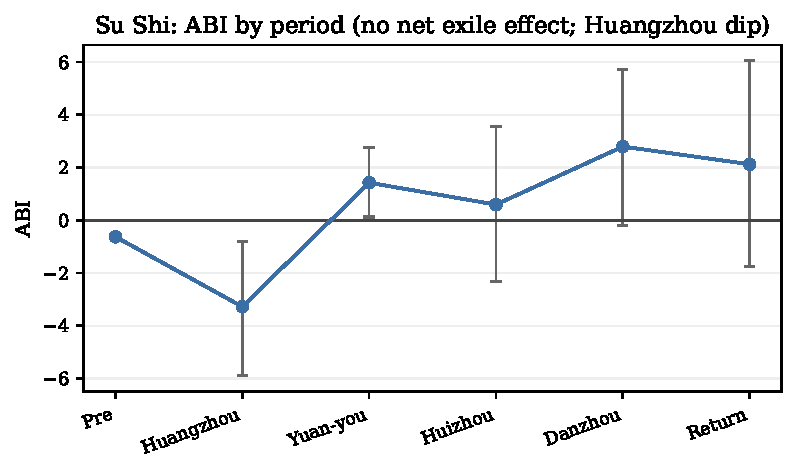
\includegraphics[width=\linewidth]{figures/fig_sushi_period.pdf}
\caption{苏轼各时期 ABI（含置信区间）；唯黄州一处深谷，整体无净贬谪效应。}
\label{fig:sushi_period}
\end{figure}图~\ref{fig:sushi_period} 显示，黄州与元祐间是仅有的两个置信区间不含零的时期（分居曲线两端），儋州则是其词汇意义上最旷达的时期（旷达闲适 $13.4$/千字，生涯峰值）。瘴疠剂量梯度 黄州(2)$\to$惠州(3)$\to$儋州(4) 逐期点估计单调，但方向与“剂量加深悲苦”模型\emph{相反}：加权线性斜率 $+3.07$/级 $[1.11,5.00]$，bootstrap $p{=}0.003$（Spearman $\rho{=}1.0$，仅 3 期，把握度低，仅作方向参考）。我们不为这一反向梯度附加任何机制解释：词表意义上苏轼的测得旷达\emph{随}贬谪严重度上升——与其自述超脱（“兹游奇绝冠平生”）一致，也与将 ABI 读作单纯“情境痛苦计”的朴素解读判然有别。稳健性方面，仅用 A 级挂接（$-0.52$）、剔除 40 字以下短诗（$+0.03$）、缓冲诗就近归期（$-0.24$），零效应结论都不变；$\pm2$ 年边界窗会清空短贬期，没有信息量，谈不上确认。

\paragraph{条件性佐证（白居易，B 级）。}白居易是唯一可做作者内切分的唐人：贬期（59 首，江州/忠州）vs 合并非贬期（84 首）得 $\Delta\mathrm{ABI}{=}{+}4.52$ $[-0.22,9.63]$——方向为正但未与零分离（双侧 $p{=}0.066$），只能作方向性佐证。这\emph{不得}读作“贬谪使他旷达”：其贬前 66 首中 50 首是新乐府讽谕诗，这一体裁让对照组浸满悲苦词汇（$12.1$ vs 贬期 $11.2$/千字），对比因此混入了体裁选择的影响。可靠的结论仅在维度层面：贬期贬谪羁旅自指（$+3.66$ $[0.83,6.54]$）与自然山水（$+24.3$ $[17.1,32.5]$，江州山水模式）显著上升。因此白居易不设 pre/post 分列，亦不进入剂量梯度。

\paragraph{其余四位官员何以不进入分析。}柳宗元无可用的贬前语料（可确知贬前诗不足 20 首）；黄庭坚可确证挂接的诗仅 4 首；欧阳修（贬期 12 首）与王禹偁（29 首）低于配对功效。我们的作者内论断因此以一份 A 级分析与一份 B 级条件性佐证为限；其余四位官员的数据不足以支撑分析。

\subsection{流传稳健性控制}
\label{sec:robust}

一位诗人的测得剖面是其所读版本的函数。我们区分两条流传渠道——\emph{重印}（共有篇目仅存传抄异文）与\emph{选本}（编者只收录全集的一个子集）——并追问各自对指数做了什么。

\paragraph{重印不改变指数。}唐侧两个来源是同一部全集的两次数字化。在 432 位共有作者上一致度为 $A{=}0.960$，五维全部保持（$S{=}5/5$；逐维 $r$ 介于 $0.95$–$0.98$），无一位作者符号翻转（图~\ref{fig:abi} 左、表~\ref{tab:tang}）。最大位移属柳宗元（$+0.22\to+0.92$）：当一位诗人的两个情感极点近乎平衡时，版本会移动一个近零差值的\emph{水平}，却不反转其符号。因此近乎完美的剖面一致（20 个"诗人×维度"格上 $r{=}0.997$）保证的是形状与次序，而非近零指数的绝对值。

\begin{table}[H]
\centering\small
\caption{唐跨版本：QTS vs.\ YD（899 卷）。$\Delta{=}|$ABI 差$|$。均值 $|\Delta|{=}0.432$；类别相关 $r{=}0.997$（20 格）。}
\label{tab:tang}
\begin{tabular}{lrrr}
\toprule
诗人 & QTS & YD & $\Delta$\\
\midrule
柳宗元 Liu Zongyuan & $+0.221$ & $+0.922$ & $0.701$\\
刘禹锡 Liu Yuxi & $-0.881$ & $-1.711$ & $0.830$\\
韩愈 Han Yu & $-2.491$ & $-2.587$ & $0.096$\\
白居易 Bai Juyi & $+1.762$ & $+1.863$ & $0.101$\\
\bottomrule
\end{tabular}
\end{table}

\paragraph{选本移动维度，不动净值。}宋侧把全集与一部独立编成的选本《御選宋詩》相比。在 253 位共有作者上（各自 $\ge300$ 字）一致度降至 $A{=}0.557$（M1 词典）/ $0.567$（语料诱导词典），属中等但明确为正的一致，五维中有三维保持 $|r|\ge0.5$（表~\ref{tab:songpop}）；选本边界削弱而非抹除作者层信号。同一批作者上的经验贝叶斯层次模型给出精确位置：净版本效应 $\hat\delta{=}+0.15$（95\% CI $[-0.31,0.59]$）\emph{含零}。但该选本带有连贯的编辑签名（表~\ref{tab:hb}）：自然山水升高 $+16.68$/千字，旷达闲适（$+1.67$）、悲苦孤寂（$+1.39$）、空幻时空（$+1.84$）同步上升（四个 CI 不含零），唯贬谪羁旅不变（$+0.05$）。指数是两极点速率之差，两极点近乎等幅同升，故在净标量上相互抵消、却在维度上清晰可见。净不变因此是抵消，而非无效应。

\begin{table}[H]
\centering\small
\caption{宋总体规模跨版本：QSS vs.\ 《御選宋詩》，253 位共有作者（两版各 $\ge$300 字）。逐维为每千字速率 Pearson $r$；数值为手工词典 / 语料诱导词典。$|r|{\ge}0.5$（保留）者标 $^*$。}
\label{tab:songpop}
\begin{tabular}{lcc}
\toprule
维度 & M1 $r$ & 诱导 $r$\\
\midrule
悲苦孤寂 Bei & $0.55^*$ & $0.59^*$\\
贬谪羁旅 Bian & $0.45$ & $0.41$\\
旷达闲适 Kuang & $0.47$ & $0.40$\\
自然山水 Zi & $0.69^*$ & $0.63^*$\\
空幻时空 Kong & $0.60^*$ & $0.61^*$\\
\bottomrule
\end{tabular}
\end{table}
\begin{table}[H]
\centering\small
\caption{经验贝叶斯层次噪声底（宋侧，253 位共享作者）。编辑效应 $\delta$ 为选本与全集净心指数的逆方差加权差；其 95\% CI 含 $0$ $\Rightarrow$ 净指数不变。逐维 $\delta_d$（每千字）暴露选本编辑签名；$^*$ 标 95\% CI 不含零者。}
\label{tab:hb}
\begin{tabular}{lcc}
\toprule
量 & 估计 & 95\% CI\\
\midrule
编辑效应 $\delta$（净指数） & $+0.15$ & $[-0.31,\,0.59]$\\
潜均值 $\mu$ & $+0.82$ & $[0.32,\,1.30]$\\
潜标准差 $\tau$ & $3.64$ & $[3.24,\,4.01]$\\
\midrule
\multicolumn{3}{l}{\emph{逐维编辑效应 $\delta_d$（每千字）}}\\
悲苦孤寂 sorrow & $+1.39^*$ & $[1.08,\,1.70]$\\
贬谪羁旅 exile & $+0.05$ & $[-0.19,\,0.28]$\\
旷达闲适 easeful & $+1.67^*$ & $[1.34,\,2.00]$\\
自然山水 nature & $+16.68^*$ & $[16.06,\,17.29]$\\
空幻时空 void & $+1.84^*$ & $[1.43,\,2.25]$\\
\bottomrule
\end{tabular}
\end{table}

\paragraph{第二部选本复现签名。}只看一次签名只是轶事。我们因此加入《宋詩鈔》（kanripo KR4h0157）——一部私家清人选本，解析得 76 位作者 9{,}612 首诗。五个维度在两部选本中\emph{同向}移动（符号 $5/5$ 一致），两条效应向量以 Pearson $0.95$ 相关（表~\ref{tab:rep}）；该相关由两本共有的自然山水位移主导（官修 $+16.7$、私家 $+4.4$/千字）。依两部选本既有选录原则事前登记的方向性预测在意象语域成立、在旷达语域不成立——两本都抬高了旷达闲适——故该签名是\emph{词典条件性}的。可复现的是编辑干预的\emph{形状}及其在意象语域的集中，而非其幅度；且它收敛在组层而非作者层：三源共有的 68 位作者上逐作者位移相关仅 $r{=}-0.11$ 至 $0.40$。净不变更只属于官修本：《宋詩鈔》把净量移离零点（$\hat\delta{=}-0.69$，95\% CI $[-1.09,-0.28]$）。跨选本可推广的是维度级签名，而非净标量的不变性。

\begin{table}[H]
\centering\small
\caption{两部各自独立编成的宋选本中的编辑签名。$\delta_d$ = 逆方差加权编辑效应（选本减全集，每千字）；$^*$ = 95\% CI 不含零。五维同号（$5/5$；n=5 无法做显著性检验，我们同时报告 $5/5$ 与 $4/5$ 一致）；$\delta$ 向量 Pearson $0.95$。右列为依选本记载的选政原则在测量前登记的方向。}
\label{tab:rep}
\begin{tabular}{lccc}
\toprule
维度 & 《御選宋詩》 & 《宋詩鈔》 & 登记方向\\
\midrule
悲苦孤寂 sorrow & $+1.39^*$ & $+1.53^*$ & up—成立\\
贬谪羁旅 exile & $+0.05$ & $+0.15$ & up—成立（幅度微小）\\
旷达闲适 easeful & $+1.67^*$ & $+0.88^*$ & 近零—不成立\\
自然山水 nature & $+16.68^*$ & $+4.43^*$ & up，小于官修—成立\\
空幻时空 void & $+1.84^*$ & $+0.03$ & 不定\\
\bottomrule
\end{tabular}
\end{table}

\paragraph{分歧落在篇目集而非文本。}以上系数把一位作者在某来源中的全部文本汇总后逐作者比较，隐含假定两渠道承载可比的篇目集。以（作者，标题）为每篇作品建键、并把每个见证重排到共同篇目边界，即可分离两种机制（表~\ref{tab:realign}）。唐侧已有 $93.3\%$ 的字落在共有篇目上，重排几乎不移动读数（$0.960\to0.966$）。三个宋侧配对仅共享 $7.5\%$、$21.6\%$、$14.2\%$ 的字——选本收录的本来就是另一批诗——然而一旦只比较两来源共有的作品，一致度一致升至 $0.90$–$0.96$。对齐并非靠压平字符串达成：QSS 与两部选本共有的作品中无一逐字节相同，平均字符相似度仅 $0.80$/$0.84$。跨版本分歧因此集中在\emph{篇目集}层，而非\emph{文本}层——这是描述性刻画，而非"文本层版本独立"的因果断言。表~\ref{tab:invariance} 汇总各一致度，图~\ref{fig:abi} 给出作者层散点；聚类作者自助（$B{=}2000$）为每个头条系数附上 95\% CI。

\begin{table}[H]
\centering\small
\caption{篇目重排对齐。\emph{汇总} = 该作者在该源中的全部文本（即前文各表口径）；\emph{对齐} = 仅取两源共有篇目（键的定义见正文）。覆盖 = 共有篇目字符量 / 汇总字符量。 95\% 置信区间来自聚类作者自助法（作者对作者重抽样 $B{=}2000$ 次）；$n$ 为进入汇总／对齐估计的作者数。}
\label{tab:realign}
\begin{tabular}{lcccr}
\toprule
对比 & 汇总 $A$ (95\% CI) & 对齐 $A$ (95\% CI) & $n$ (汇总/对齐) & 覆盖率\\
\midrule
唐：QTS vs.\ YD（同书两数字化） & $0.960\,[0.948,0.971]$ & $0.966\,[0.957,0.974]$ & $432/415$ & $0.932$\\
宋：QSS vs.\ 《御選宋詩》 & $0.557\,[0.459,0.647]$ & $0.899\,[0.853,0.936]$ & $253/179$ & $0.075$\\
宋：QSS vs.\ 《宋詩鈔》 & $0.822\,[0.630,0.921]$ & $0.957\,[0.924,0.979]$ & $75/73$ & $0.216$\\
宋：《御選宋詩》 vs.\ 《宋詩鈔》 & $0.634\,[0.460,0.768]$ & $0.961\,[0.896,0.987]$ & $68/51$ & $0.142$\\
\bottomrule
\end{tabular}
\end{table}
\begin{table}[H]
\centering\small
\caption{各源对跨版本一致性。$A$ = 一致性（净 ABI 的 Pearson $r$）；$S$ = 结构一致性（$|r|{\ge}0.5$ 的五维比例）。所有对均取两源各 $\ge$300 字作者；末两行进一步限制在全部三源宋本共有的 68 位作者，使两选本可比。 汇总口径三个核心系数的自助 95\% 置信区间分别为 $[0.948,0.971]$（唐）、$[0.459,0.647]$（QSS/御選）、$[0.630,0.921]$（QSS/宋詩鈔），均显著大于零。}
\label{tab:invariance}
\begin{tabular}{lcccr}
\toprule
对比 & 词典 & $n$ & $A$ & $S$\\
\midrule
唐：QTS vs.\ YD（同书） & M1 & 432 & $0.960$ & $5/5$\\
唐：QTS vs.\ YD（同书） & 诱导 & 432 & $0.938$ & $5/5$\\
宋：QSS vs.\ 御選（选本） & M1 & 253 & $0.557$ & $3/5$\\
宋：QSS vs.\ 御選（选本） & 诱导 & 253 & $0.567$ & $3/5$\\
宋：QSS vs.\ 宋詩鈔（选本） & M1 & 75 & $0.822$ & $5/5$\\
宋：QSS vs.\ 御選，共有作者 & M1 & 68 & $0.601$ & $4/5$\\
宋：QSS vs.\ 宋詩鈔，共有作者 & M1 & 72 & $0.827$ & $5/5$\\
\bottomrule
\end{tabular}
\end{table}
\begin{figure}[t]
\centering
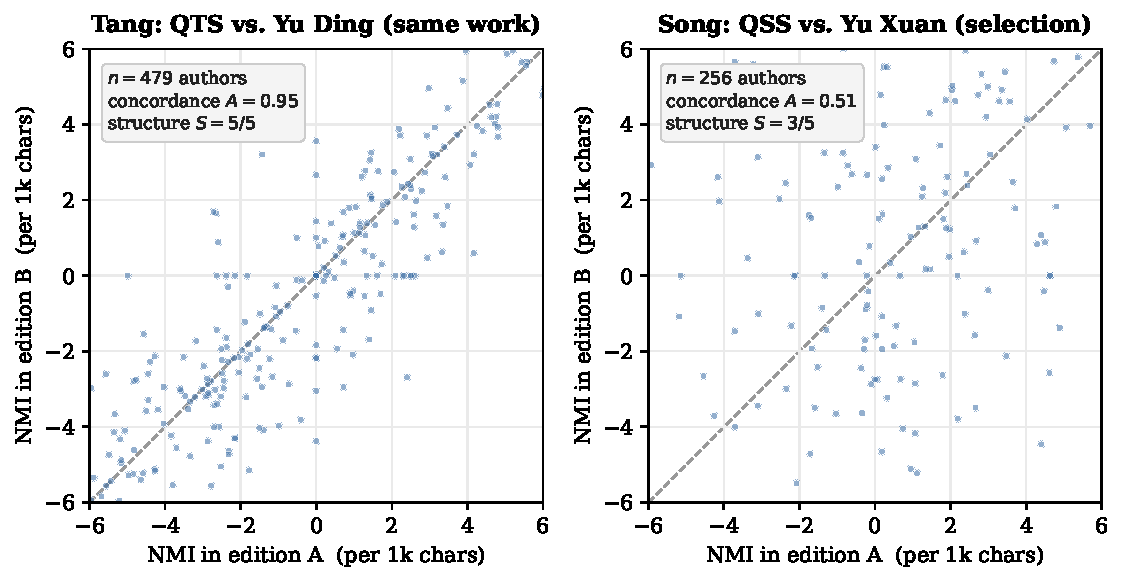
\includegraphics[width=\linewidth]{figures/abi_cross_edition.pdf}
\caption{流传稳健性控制，每点为一个共享作者（版本 A vs 版本 B 的净心指数；虚线为完美一致）。
\textbf{左：}唐，《全唐诗》vs.\ 《御定全唐诗》——同一著作的两次数字化；432 位作者紧密沿对角线（$A{=}0.960$，$S{=}5/5$）。
\textbf{右：}宋，《全宋诗》vs.\ 官修《御選宋詩》选本——另一部著作；253 位作者形成明显更松散的云（$A{=}0.557$，$S{=}3/5$）。选本移动个体分数而不产生系统性净偏移（表~\ref{tab:hb}、\ref{tab:rep}），故云松散却不漂移。第二部宋选本以表~\ref{tab:rep} 数值报告。}
\label{fig:abi}
\end{figure}

\paragraph{反事实渠道。}把每位作者的维度速率后验投影到各渠道，可量化剖面中属于幸存版本的部分。总体层每条渠道的偏移都远小于作者间异质（$\tau\approx3.6$）：官修 $+0.15$、私家 $-0.68$、唐重印 $-0.04$。五维剖面则是另一番景象（图~\ref{fig:counterfactual_delta}）：两部选本同向抬高每一维，自然山水最甚，净效应之所以小只因两极点抵消。作者层的不对称随之具体化：陆游（$+0.57$）、苏轼（$+0.41$）、欧阳修（$-0.18$）在私家渠道下均改变符号，而秦观的枯槁（$-2.11$ / $-1.56$ / $-2.72$）与王禹偁的近中性则跨渠道保持。256 位宋人作者的整体排序稳定（全集实测与官修反事实的 Spearman $=0.96$），但 $13.6\%$ 的两两序对翻转、26 位作者的位移 CI 不含零，而零下期望约 13 位。唐重印渠道则主要以共模方式位移、基本不重排作者：刘禹锡的反事实（$-1.26$）介于其两版本测值（$-0.88$、$-1.71$）之间。作者级\emph{重塑}是选本的属性；对宋人而言，流传渠道是一位可见的、维度特异的合著者。

\begin{figure}[t]
\centering
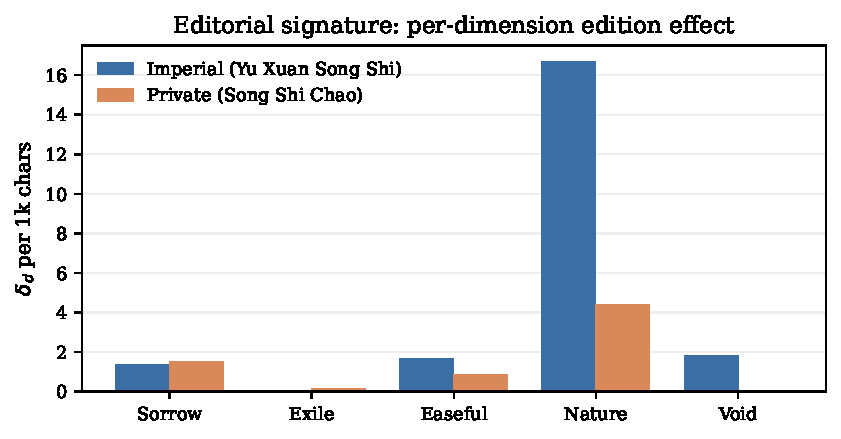
\includegraphics[width=\linewidth]{figures/fig_counterfactual_delta.pdf}
\caption{两部选本在五个维度上同向偏移，自然山水维度主导（官修 $+16.7$、私家 $+4.4$ 每千字）。}
\label{fig:counterfactual_delta}
\end{figure}

\section*{局限}
\begin{itemize}
\item (a) 作者级效标 $r{=}0.57$ 校验的是短诗金标子样本，而非表~\ref{tab:abi} 的全集值。
\item (b) CNN 仅恢复两情感极（悲苦孤寂、旷达闲适），其余三维在预测中持平于零。
\item (c) 256 位作者中 26 位 CI 跨零，而零下期望约 13 位。
\item (d) 辛弃疾等小语料作者未经版本控制，其定位仅建立在全集语料之上。
\end{itemize}

\section{结论}
\label{sec:conclusion}

本文为唐宋贬谪诗歌的情感测量提供了一套可复现的仪器，并据此把十二位具名贬谪官员放到
同一标尺上比较。仪器是一个字符级卷积网络，直接从原始字符预测一部透明五维词典的标量净
心指数（$r{=}0.934$）；其结果把枯槁者（韩愈、秦观）与明确闲适者（白居易、黄庭坚、范
仲淹、辛弃疾）分开，其余五人与中性无统计差异。词表扰动检验进一步区分二者：六个近零定
位的符号翻转率高于 $20\%$，读作完整词表下的条件性结论；六个明确极性的定位则在至少
$90\%$ 的扰动轮次中保持符号（表~\ref{tab:abi}）。由于网络以该词典为训练目标，它与人工
盲标的一致（诗级 $\rho{=}0.46$、作者级 $r{=}0.57$）是对词典效度的上界，而非独立检验；
指数在维度间负载不均——定义它的旷达极仍居最弱一端（$0.29$）。五类语域容纳不下反讽与
依赖用典的情感；从分析器残差中恢复的三个语域（静禅、思乡、羁旅行役）经盲标验证后并入
词表（\S\ref{app:lexicon}）。

第二项贡献属于测量论。一位诗人的分数是其所读版本的函数：同一部唐集的两次数字化几乎不
改变测量（$A{=}0.960$），而两部独立编成的宋选本以一致的维度级模式抬高意象与闲适词汇
——净指数在官修本上存活、在私家本上偏移。跨版本分歧集中在编者所选的\emph{篇目集}，而
非任何一首诗的文本，故从单一版本报告的情感分数部分地是一个编辑决定。同一框架还给出反
事实投影，把测得剖面归因到各流传渠道；以及苏轼的作者内分析——未发现净贬谪效应，旷达词
汇反而随贬谪加深而上升，仅三期，作为与“贬谪致郁”通说并列参看的量化观察呈报，而非对其
的修订。

仪器的限度为实测所得：金标规模有限且与词典出自同一语料家族；选本检验只覆盖两部宋代
《四库》系统选本；语料限于诗体。


所有文本皆为公有领域古典作品；不涉及个人或非公开数据。量化分数意在补充而非取代人文学科的细读。

\section*{数据与代码可用性}
\label{sec:repro}
所有来源皆为公有领域古典作品。语料：《全唐诗》《全宋诗》（Book1Q84 / 中文文本库数字版，2025 年快照）及两种 kanripo 对康雍乾选本的转录（KR4h0143《御選宋金元明四朝詩》\citep{kangxi1709}；KR4h0157《宋詩鈔》\citep{wu1671}），皆属《四库全书》文渊阁本；版本与快照标识记录于随附仓库。测量仪器与全部分析脚本随投稿提供，含去标识的双编码原文（\texttt{annotations/}）与从原始语料重算本文每一数字、写出 \texttt{numbers\_ledger.json} 的编排器 \texttt{recompute\_all.py}（将每项报道量映射到源脚本与结果键）。每处随机步骤固定种子（NumPy、\texttt{random}、\texttt{torch.manual\_seed}）；稿件以 \texttt{xelatex} 编译以处理中文字形。全部深度学习实验在单台工作站完成（CPU 训练，PyTorch~2.14.0+\texttt{cpu}；中文文本以 OpenCC 规整），精确版本钉于随附仓库的 \texttt{requirements.txt}。

\bibliographystyle{plainnat}
\begin{thebibliography}{9}
\bibitem[Kim(2014)]{kim2014convolutional}
Y.~Kim.
\newblock Convolutional neural networks for sentence classification.
\newblock In \emph{EMNLP}, 2014.

\bibitem[Stamatatos(2009)]{stamatatos2009survey}
E.~Stamatatos.
\newblock A survey of modern authorship attribution methods.
\newblock \emph{Journal of the American Society for Information Science
and Technology}, 60(3):538--556, 2009.

\bibitem[Hou and Frank(2015)]{hou2015sentiment}
Y.~Hou and A.~Frank.
\newblock Analyzing sentiment in classical Chinese poetry.
\newblock In \emph{Proc.\ of the 3rd Workshop on Language Technology for
Cultural Heritage, Social Sciences, and Humanities (LaTeCH)}, 2015.

\bibitem[Du et al.(2025)]{du2025multimodal}
X.~Du, H.~Pei, and H.~Zhang.
\newblock Picturized and Recited with Dialects: A Multimodal Chinese
Representation Framework for Sentiment Analysis of Classical Chinese
Poetry.
\newblock \emph{arXiv preprint arXiv:2505.13210}, 2025.

\bibitem[Liu and Zhao(2025)]{liu2025samcap}
Z.~Liu and W.~Zhao.
\newblock Sentiment analysis of Chinese ancient poetry based on multidimensional
attention under the background of digital intelligence integration.
\newblock \emph{Libri}, 75(1):97--108, 2025. DOI: 10.1515/libri-2024-0053.

\bibitem[Qin et al.(2025)]{qin2025shades}
Z.~Qin, S.~Ng, and Y.~Song.
\newblock Shades of grey: Quantifying a database of 18 aesthetic moods in
classical Chinese poetry.
\newblock \emph{Empirical Studies of the Arts}, 43(2):1181--1213, 2025.
DOI: 10.1177/02762374241305561.

\bibitem[Zhou et al.(2022)]{shiziren2022}
A.~Zhou, C.~Sang, Y.~Zhang, and M.~Lu.
\newblock 诗人密码: 唐诗作者身份识别 (The Poet Code: Tang Poetry Authorship
Identification).
\newblock \emph{Journal of Chinese Information Processing
(中文信息学报)}, 36(6):162--170, 2022. DOI: 10.3969/j.issn.1003-0077.2022.06.017.

\bibitem[Zhou et al.(2021)]{zhou2021lda}
A.~Zhou, Y.~Zhang, H.~Wei, and M.~Lu.
\newblock LDA-Transformer Model in Chinese Poetry Authorship Attribution.
\newblock In \emph{Information Retrieval: 27th China Conference, CCIR 2021,
Dalian, China, October 29--31, 2021, Proceedings (LNCS, vol.~13026)}, pages
59--73. Springer, 2021. DOI: 10.1007/978-3-030-88189-4\_5.

\bibitem[Fang(2011)]{fang2011cld}
A.~C.~Fang, W.-y.~Li, and J.~Cao.
\newblock In search of poetic discourse of classical Chinese poetry: an
  imagery-based stylistic analysis of Liu Yong and Su Shi.
\newblock \emph{Chinese Language and Discourse}, 2(2):232--249, 2011.
  John Benjamins. DOI: 10.1075/cld.2.2.04fan.

\bibitem[Yuan et al.(2023)]{yuan2023variants}
L.~Yuan, D.~Wang, and S.~Huang.
\newblock Automatic discovery of parallel textual variants in classical
Chinese texts.
\newblock \emph{Journal of Library Science in China (图书情报工作)} /
ChinaXiv: chinaxiv-202304.00607, 2023.

\bibitem[Song et al.(2022)]{bianzhe2022}
X.~Song, X.~Huo, Y.~Liu, and J.~Deng.
\newblock 数字人文视角下《全唐诗》贬谪诗人的时空轨迹分析 (Spatiotemporal
Trajectory of Exiled Poets in the Complete Tang Poems).
\newblock \emph{Library and Information Service (图书情报工作)}, 66(7):26--34,
2022. DOI: 10.13266/j.issn.0252-3116.2022.07.003.

\bibitem[Wang and Zhu(2023)]{wang2023lideyu}
Q.~Wang and T.~Zhu.
\newblock Use data for education: Li Deyu's self-reported texts of two
demotions as an example.
\newblock In \emph{Proc.\ of ICAIE}, Atlantis Press, 2023.
DOI: 10.2991/978-94-6463-242-2\_36.

\bibitem[Wang and Sun(2008)]{wang2008finding}
王兆鹏, 孙凯云.
\newblock 寻找经典——唐诗百首名篇的定量分析.
\newblock 《文学遗产》, 2008(2):40--52.

\bibitem[Shang(2007)]{shang2007exiled}
尚永亮.
\newblock 《唐五代逐臣与贬谪文学研究》.
\newblock 武汉大学出版社, 2007.

\bibitem[Xing(2024)]{xing2024liusu}
邢若琳.
\newblock 论柳宗元、苏轼流寓心态之异同.
\newblock 《今古文创》, 2024(36):52--55.

\bibitem[Kangxi(1709)]{kangxi1709}
康熙 (Kangxi Emperor), 御定.
\newblock 御選宋金元明四朝詩 (Yu Xuan Song Jin Yuan Ming Si Chao Shi).
\newblock Imperial anthology, 1709. Transcription: kanripo KR4h0143
(\emph{Siku Quanshu} base edition).

\bibitem[Wu(1671)]{wu1671}
吳之振 (Wu Zhizhen), 編.
\newblock 宋詩鈔 (Song Shi Chao).
\newblock Private anthology, Qing dynasty; \emph{Siku Quanshu} Wenyuange text,
106 \emph{juan}. Transcription: kanripo KR4h0157 (\emph{Siku Quanshu} base
edition).

\bibitem[Lou and Yu(2025)]{overlock2025}
M.~Lou and Y.~Yu.
\newblock OverLoCK: An Overview-first-Look-Closely-next ConvNet with
Context-Mixing Dynamic Kernels.
\newblock In \emph{Proc.\ of the IEEE/CVF Conference on Computer Vision and
Pattern Recognition (CVPR)}, 2025 (Oral). arXiv:2502.20087.

\bibitem[Lou et al.(2025)]{transxnet2025}
M.~Lou, S.~Zhang, H.-Y.~Zhou, S.~Yang, C.~Wu, and Y.~Yu.
\newblock TransXNet: Learning Both Global and Local Dynamics with a Dual Dynamic
Token Mixer for Visual Recognition.
\newblock \emph{IEEE Transactions on Neural Networks and Learning Systems
(TNNLS)}, 2025. arXiv:2310.19380.

\bibitem[Cai et al.(2026)]{pfgn2026}
X.~Cai, C.~Sun, Y.~Wang, H.~Yang, and Y.~Wu.
\newblock PFGNet: A Fully Convolutional Frequency-Guided Peripheral Gating
Network for Efficient Spatiotemporal Predictive Learning.
\newblock In \emph{Proc.\ of CVPR}, 2026. arXiv:2602.20537.

\bibitem[Hsing and Tu(2026)]{tacnn2026}
C.-W.~Hsing and W.-L.~Tu.
\newblock Tensor-Augmented Convolutional Neural Networks: Enhancing Expressivity
with Generic Tensor Kernels.
\newblock \emph{arXiv preprint arXiv:2604.08072}, 2026.

\bibitem[Farvardin and Chapman(2026)]{facnn2026}
P.~Farvardin and D.~Chapman.
\newblock End-to-end Feature Alignment: A Simple CNN with Intrinsic Class
Attribution.
\newblock \emph{arXiv preprint arXiv:2603.25798}, 2026.

\end{thebibliography}

\appendix

\section{选本的转录与解析}
\label{app:parse}
《御選宋詩》仅以《御選宋金元明四朝詩》（kanripo KR4h0143）的 mandoku 纯文本存世，其中 78 卷宋诗与作者名录、序文以及少量金、明之卷交错混排。本文解析每一行\emph{诗}正文（缩进最低者），并以（简体）作者名与《全宋诗》8{,}925 人的作者名录精确匹配，将其归入所属作者；由此得到 660 位作者的 9{,}405 首诗，且全 660 位都能在 QSS 中找到对应作者，可证解析正确。《宋詩鈔》按同一方式转录：正文取缩进最低者，每位诗人的段落以其\emph{集名行}锚定——包括把欧阳修、王安石、苏轼分置于数卷的 上/中/下续卷行——而紧接集名行之后、习惯性附于书首的散文\emph{小传}予以剔除、不计入诗，因为小传惯于叙述贬谪与迁转，若计入，只会在选本一侧抬高贬谪羁旅与悲苦孤寂两个语域。该解析锚定 98 个集名行，得到 76 位作者的 9{,}612 首诗、诗句 829{,}341 字，无未能归位的集名行。

该文本有两项已载于文献的特征，直接关系到这项比较应如何阅读。其一，《四库》提要记载，它所列诗人中有十六家在本副本中“有録無書”——“蓋剞劂未竣故竟無完帙也”（仅存目录而无正文，因刻工未竟），并把全书所收记为百家。若此数精确，此本的完整形态应有八十四位诗人有诗，而本文恢复出 76 位，尚余八家既未被锚定、也无法搪塞过去。这一缺口只影响作者的\emph{覆盖}，不影响已恢复诗人的逐作者比率；$\delta$ 又只在两侧同时存在的作者上计算，故不因此直接产生偏倚。其二，同一提要还记载，因每位诗人各自为集、“甫刋一帙即摹印行世”，故“所傳之本往往多寡不同”——同一部选本的传世诸本，其所含多寡常常互异。这恰是本文的论点由清代编者亲口说出：对一部选本而言，“版本”在任何测量开始之前就已不是一个稳定对象，而本文所用的《四库》本只是诸本之一。

\section{作者 / 朝代 / 散文归属}
\label{app:attr}
本附录报告归属任务，它与“情感测量是否可信”是\emph{不同}的问题——辨认\emph{谁}写了某诗，不同于测量作者\emph{感受如何}——故置于主线之外。古典诗歌作者归属研究已多：唐诗作者识别的 Cap-Transformer 模型 \citep{shiziren2022}、LDA-Transformer 混合 \citep{zhou2021lda}、以及区分柳永与苏轼的意象风格特征 \citep{fang2011cld}。本文复用同一特征仅作补充性探测。

本文在相同的 85/15 分层划分上比较了三类分类器：字符级 CNN \citep{kim2014convolutional}（embedding + conv + max-pool，128 维末层）、字符 $n$-元组 TF-IDF 加逻辑回归、以及同一特征加线性 SVM。所有随机过程共享单一固定种子（\texttt{SEED}${=}20260915$）。表~\ref{tab:attr} 显示轻量的 TF-IDF + 线性 SVM \emph{优于}字符级 CNN 于每一任务，且更易复现、无需 GPU。12 路作者任务受严重类不平衡所限（次要作者 154–320 首，主要作者 2{,}000+），macro-F1 虽低而 weighted-F1 高，反映类不平衡对逐类绩效的制约。

\begin{table}[H]
\centering\small
\caption{归属：准确率 / macro-F1。每行最优以粗体标出。}
\label{tab:attr}
\begin{tabular}{lccc}
\toprule
任务 & CNN & TF-IDF+LR & TF-IDF+SVM\\
\midrule
作者（12） & .624/.271 & .714/.351 & \textbf{.802/.568}\\
朝代（2） & .894/.837 & .895/.808 & \textbf{.936/.898}\\
唐文（4） & .619/.512 & .856/.812 & \textbf{.924/.908}\\
\bottomrule
\end{tabular}
\end{table}

\section{跨版本不变表示探测（M6）}
\label{app:m6}
作为一项探测——而非核心论断——我们问：一个\emph{学得的}表示能否在剥离版本特有泄漏的同时，保住诗人的情感？我们冻结 PPMI–SVD 分解的字符嵌入（\texttt{classical\_ppmi\_svd.npz}；100 维、行单位范数），以每诗字符向量均值表示诗，取每作者在\emph{两}版本中皆 $\ge$300 字者的作者均值 100 维向量；情感读出与 \S\ref{sec:robust} 完全相同：将每作者向量投影到五个词典极点方向得 5 维信号，并算 $(A,S)$。我们以闭式域对抗解得一线性“源不变”投影 $g:\mathbb{R}^{100}\!\to\!\mathbb{R}^{100}$：训练逻辑对抗器从作者均值向量预测版本，其权 $\mathbf w$ 即版本可判别方向，将该方向投影出去
$g(\mathbf x)=\mathbf x-(\mathbf x\!\cdot\!\mathbf w)\mathbf w$，恰移除版本轴——此构造对此目的最优。本文在汇总的跨版本作者对上训练了一个共享投影，并施于两种设定。

\begin{table}[H]
\centering\small
\caption{M6 不变表示探测。Frozen = PPMI–SVD 作者均值骨干上的恒等投影；M6 = 闭式域对抗投影。$A$/$S$ 为从 5 维极点投影读出的 一致性系数。edAUROC = 5 折逻辑版本可预测性（越低越不变）；varR = M6 保留的维度方差比（$1.0$ = 未移除）。}
\label{tab:m6}
\setlength{\tabcolsep}{3.2pt}
\begin{tabular}{lcccccc}
\toprule
设定 & $n$ & 变体 & $A$ & $S$ & edAUROC & varR\\
\midrule
唐：QTS vs.\ YD & 363 & frozen & $0.865$ & $1.00$ & $0.536$ & $1.00$\\
唐：QTS vs.\ YD & 363 & M6 & $0.981$ & $1.00$ & $0.537$ & $0.69$\\
\midrule
宋：QSS vs.\ YXSS & 216 & frozen & $0.900$ & $1.00$ & $0.848$ & $1.00$\\
宋：QSS vs.\ YXSS & 216 & M6 & $0.980$ & $1.00$ & $0.584$ & $0.49$\\
\bottomrule
\end{tabular}
\end{table}

唐同书对上版本方向本就微小（edAUROC $0.536$ $\approx$ 随机），故 M6 几无可移除，情感读出不变。宋选本对上版本方向巨大且主导：冻结表示高度可预测版本（edAUROC $0.848$），M6 恰移除该轴，把版本可预测性压至 $0.584$，同时保留全部五维情感（$S{=}1.00$）并将 $A$ 由 $0.900$ 升至 $0.980$。本文将此作为\emph{探测}并附明确告诫：其 $A$/$S$ 与表~\ref{tab:invariance} \emph{不可直接比}，其唯一被许可的解读是定性的——这些表示中的版本信息是一条单一、低秩、可分离的方向，可移除而不损情感维度。这与主线发现一致：版本效应沿特定方向作用，而非弥散噪声。

\section{五维“情绪—意象”词典}
\label{app:lexicon}
词典 $\mathcal{L}$ 把词划分入五类，下录\emph{全部}条目。每类混列单字与多字词；全部条目以简体存储，与语料的归一化（繁$\to$简经 OpenCC）一致。两个情感性极点标 (A)；主题性的贬谪羁旅类（指境况而非感受）另行标 (A$^\dagger$)；两类意象语域标 (I)。

\smallskip
\noindent\textbf{悲苦孤寂} \textsc{Bei} (A；sorrow–loneliness)：
悲 伤 愁 怨 苦 孤 寂 独 凄 惨 哀 痛 恨 忧 戚 惘 怆 涕 泪 殇 殁 愍 悴 惸 黯 销 魂 零 萧 雁 砧 捣 吏 灯 店 舫 猿 驿 帆 仆 僮
断肠 凄凉 寂寥 孤危 憔悴 销魂 悲秋 苦辛 酸辛 辛酸 飘零 飘蓬 断蓬 飞蓬 转蓬

\smallskip
\noindent\textbf{贬谪羁旅} \textsc{Bian} (A$^\dagger$；exile–journey，指境况而非感受)：
贬 谪 迁 逐 流 羁 旅 客 宦 远 荒 蛮 瘴 殊 遐 徼 陬 裔
去国 天涯 海角 殊方 投荒 远谪 迁客 楚客 南荒 炎荒 瘴江 蛮烟

\smallskip
\noindent\textbf{旷达闲适} \textsc{Kuang} (A；detached–easeful)：
闲 适 达 旷 豁 放 醉 啸 傲 悠 淡 泊 乐 欣 悦 遣 兀 疏 狂 从 容 恬 静 禅 苔 钓 隐 亭 栽 莲 畦 眠
旷达 闲适 放达 自适 陶然 悠然 忘机 委运 随遇 达观 适意

\smallskip
\noindent\textbf{自然山水} \textsc{Zi} (I；nature–landscape)：
山 水 风 月 林 泉 石 竹 松 江 河 湖 海 花 鸟 溪 岩 岚 汀 洲 屿 峰 崖 涧 泽 涯 渚 苹 蓼
清风 明月 白云 沧浪 烟霞 苇岸 渔樵 桃源 落英 幽篁 暮云 孤云 寒云 春云 秋云 停云 烟云 云霞 云峰 云山

\smallskip
\noindent\textbf{空幻时空} \textsc{Kong} (I；void–temporality)：
空 幻 梦 影 尘 虚 浮 瞬 逝 昔 古 千 秋 万 须 臾 泡 电 光 隙 驹 阴
浮生 如梦 梦幻 须臾 万古 古今 今古 泡影 微尘 刹那 弹指 过眼 逆旅 倏忽

\smallskip
\noindent\textbf{词典的语料覆盖。}
表~\ref{tab:lexfreq} 报告每类在统合\emph{诗}层（21{,}287 首、1{,}466{,}827 字）上的触发频率。五类触发充分且相对均衡；自然山水如预期最频繁，反映景观在古典诗中的中心地位。

\begin{table}[H]
\centering\small
\caption{词典语料覆盖（统合\emph{诗}层）。}
\label{tab:lexfreq}
\begin{tabular}{lrrrr}
\toprule
类别 & 条目 & 命中 & 命中诗 (\%) & 每千字速率\\
\midrule
悲苦孤寂 Bei & 56 & 18,677 & 10,303 (48.4\%) & 12.73\\
贬谪羁旅 Bian & 30 & 9,549 & 6,721 (31.6\%) & 6.51\\
旷达闲适 Kuang & 43 & 19,446 & 11,054 (51.9\%) & 13.26\\
自然山水 Zi & 49 & 45,254 & 16,478 (77.4\%) & 30.85\\
空幻时空 Kong & 36 & 26,442 & 13,308 (62.5\%) & 18.03\\
\bottomrule
\end{tabular}
\end{table}

\noindent 净心指数为
$\mathrm{ABI}(a)=\phi_{a,\textsc{Kuang}}-\phi_{a,\textsc{Bei}}$
（式 2）。

\noindent 静禅语域由旷达类的禅/苔/钓/隐/亭/栽/畦/眠承载；羁旅与思乡语域由悲苦类的驿/帆/舫/店/灯/砧/捣/仆/僮承载（词条数见 \texttt{results\_lexicon\_v2\_curation.json}：悲苦孤寂 37→47→56、旷达闲适 33→43）。

\section{贬谪编年与诗级分期挂接协议}
\label{app:chron}
四库语料均不携带诗级年代元数据（QTS/QSS/YD/YXSS 共 356{,}714 首中可用年代字段为 0；唐库 \emph{tags} 为主题标签、宋库 \emph{strains} 为平仄标记，均非系年），故作者内分期须外挂编年注释层。我们依通行学术成果（正史、年谱、编年注本）为每位队列官员编制贬谪事件表，逐条标注依据等级：A（正史与编年一致）、B（学界通行）、C（有争议，永不并入 A/B）。诗级挂接走两条路线：其一，内部编年次序并以锚点诗校验（苏轼《全宋诗》序列自首篇起即为编年——乌台狱中诗、《初到黄州》《别黄州》《初到惠州》、海南诸诗至绝笔严格递增；绝笔之后的补编区非编年，标 \emph{unknown}）；其二，对分体杂编的别集，依编年注本逐首挂接。每条事件边界 $\pm1$ 年设缓冲期，不参与任何对比。覆盖率：苏轼 473 贬期 / 995 贬前 / 860 贬后（全集 85\% 为 A 级挂接）；白居易 59 / 66 / 18（B 级，附体裁选择偏差声明）；其余四人挂接后低于配对功效（刘禹锡贬期 42 首而无可分的 pre/post 对照；欧阳修 12；王禹偁 29；黄庭坚 4）。挂接表、依据等级与覆盖率随复现包发布（\texttt{poem\_period\_labels.csv}、\texttt{exile\_chronology.csv}）。

\section{金标标注协议与复现控制}
\label{app:goldrep}

\paragraph{抽样。}
金标样本为 160 首\emph{诗}，每代 80 首，按朝代、是否属十二人队列、以及诗之词典 ABI 在中位数上下之交叉做分层随机抽样（种子 20260917）；每代 60 首来自全集、20 首来自选本，使样本跨越两种流传机制与仪器输出的全幅而非仅中部。诗限制在 20–160 字：低于 20 字每千字速率无意义，高于 160 字则逐首盲标双编码负担过重。实现样本覆盖 78 位作者。编码者以固定随机序收到诗作，隐去作者、题名、朝代、选本归属与全部词典输出，故编码不能锚定于既有声望。

\paragraph{仪器与信度。}
每诗在五维 0–3 序数量表上评分（0 = 无，1 = 偶一出现，2 = 明显存在，3 = 主导），类别定义见 \S\ref{app:lexicon}，编码前就每类商定两例锚；两编码者独立评完全部 160 首，不以讨论消歧，故信度数字未被共识抬高。信度报为二次加权 $\kappa$、序次 Krippendorff $\alpha$ 与 ICC$(2,1)$，金标指数取编码者均值，与式 (2) 完全相同。

\paragraph{为何折半在此取连续而非奇偶。}
诗的逐首信度通过对每诗字符前后半分别施词典、并报所得相关的 Spearman–Brown 校正来算。按交替字符切分会切断每个二元组与对仗，使相关因与分词仪器有效性无关之因而归零；故该估计在构造上保守，其近零值应读作“诗级词频稀疏”的声明，而非词典设计问题。同一告诫适用于 $|\widehat{\rho}|$：在 40 字诗中仅触发数次的词典，无论其聚合表现如何，皆不可能在该单元上可靠。

\paragraph{金标敏感度与逐作者一致。}
删去短于 28 字的诗（$n{=}150$）、删去极端 5\% 词典分数（$n{=}147$）或删去最长诗（$n{=}150$），聚合相关分别为 $0.43$、$0.38$、$0.40$，各带 95\% CI，确认聚合相关非由任何诗子集驱动。逐作者一致更弱：在至少三首被抽样诗的十位金标作者上，一致为 $\rho{=}0.13$（95\% CI $[-0.55,0.69]$，$n{=}10$），该样本量下与无差异难分。金标仅限\emph{诗}；此处无任何许可将分析器用于\emph{词}或散文。

\end{document}
